\documentclass[twocolumn,conference]{article}

\usepackage{amsmath,amssymb,amsfonts}
\usepackage{xcolor}
\usepackage{listings}
\usepackage{inputenc}
\usepackage{graphicx}
\usepackage{authblk}
\usepackage{enumerate}
\usepackage{caption}

\usepackage{array,booktabs,longtable,tabularx}
\usepackage{ltablex}
\usepackage{wrapfig,lipsum,booktabs}
\usepackage{multirow}

\providecommand{\keywords}[1]
{
  \small	
  \textbf{\textit{Keywords---}} #1
}

\begin{document}
\author[1]{Eric Raphael Huiza Pereyra}
\affil[1]{Pontifical Catholic University of Peru}
\affil[]{\textit{eric.huiza@pucp.edu.pe}}

\author[2]{Cesar Augusto Olivares Poggi}
\affil[2]{Pontifical Catholic University of Peru}
\affil[]{\textit{cesar.olivares@pucp.edu.pe}}

\title{%
	\vspace{-2.0cm}
	\textbf{Talking with signs} \\	
	\Large \textbf{A method for detecting signs in a weakly annotated dataset}
}

\maketitle
    
\begin{abstract}
People with deafness or hearing disabilities who aim to use computer based systems, state of art video classification and human action recognition rely in a combination of traditional and new methods like optical flow and 3D CNN. In this article we show a novel method to detect Peruvian Sign Language elements (nSDm) from a weakly annotated videos dataset. Video annotation techniques were applied increasing the models performance, as a result we achieved XX precision and XX exhaustiveness by training a 3D CNN with optical flow inputs.   \\
\keywords{video classification,human actions detection, optical flow, 3D CNN.}
\end{abstract}

\section{Introduction}\label{intro}

The World Health Organization (WHO) stated that 466 million people world wide have disabling hearing loss, estimating that by 2050 over 900 million people will have disabling hearing loss and will represent a global cost of 750 million dollars annually \cite{deafness_and_hearing_loss_2019}. 

The Peruvian Institute of Informatics and Statistics (INEI) conducted a national disabilities survey with the objective of segmenting and better understanding which disabilities affect the Peruvian population \cite{disabilities_survey_2012}, the results showed that 1.8\% of the Peruvian population suffer at least partial when not permanent deafness or hearing limitation. 

As of today, thanks to deep learning models for computer vision and natural language processing, it is completely feasible to propose systems able to detect and transcribe sign languages. However, deep learning supervised models usually require large and well annotated datasets, and developing such a dataset for the Peruvian Sign Language (PSL) \cite{lsp_2015} is expensive and difficult to achieve. Furthermore, in the same way as spoken languages, signs languages also present local variations e.g. people who live in Lima metropolitan area are not expected to use the same set of signs as people leaving in other parts of the country. A need exists for approaching this task with self-supervised learning or by means of weakly labeled data.

This article reports research conducted with the goal of proposing a method for detecting PSL signs using a weakly annotated dataset, and answering the following research questions:

\begin{enumerate}[(i)]
\item What are most relevant currently available techniques for training an AI model from  weakly annotated video and audio transcription?\label{q1}
\item How precise and exhaustive is the model described in the above question on the recognition of a reduced set of signs in a weakly annotated dataset?\label{q2}
\item What is the relation between the number of samples and the detection of new LSP elements in terms of nSDm precision and recall?\label{q3}
\end{enumerate}

The Pontifical Catholic University of Peru (PUCP) Grammar and  Signs research group created a PSL dataset \cite{lsp_dataset} that is weakly annotated because it does not show exactly the relation between the instant when a sign that is emitted and its corresponding translation.

nSDm will take advantage of the PSL dataset \cite{lsp_dataset} and will contribute with the generalization and progressive signs detection that could be used as a starting point for future studies including software accessibility improvements and human computer interaction for people with deafness and hearing limitations.

The rest of the article is organized as follows. In sec \ref{relatedwork} we review the related work on video classification and body actions recognition using both Optical Flow+Two Stream CNN and 3D CNN architectures. In sec \ref{method} we introduce nSDm and specify its architecture and design. In sec \ref{experimentation} we evaluate nSDm precision and recall and provide answers for the research questions \ref{q1},\ref{q2},\ref{q3}. In sec \ref{datasetdesc} we describe and provide the dataset details. In sec \ref{videoannot} we describe the video annotation and data pre-processing techniques applied to the dataset and finally in sec \ref{conclusion} we present our conclusion and describe future work.
\section{Related Work} \label{relatedwork}
\subsection{Action Recognition}
Human action recognition is a extensively studied field, action recognition dataset like UCF101, HMDB51, THUMOS14  are available, researches tried to solve the human action recognition problem using different approaches including Optical Flow and 3D CNN \cite{qiu2017learning}.  \textbf{Optical Flow,} is defined as the pattern obtained from the motion of objects, surfaces and edges in a visual scene caused by the relative motion between the observer and a scene, it is achieved by distributing movement velocities and brightness across frames. It is a  key concept in action recognition from videos \cite{wang2019hallucinating}. Optical flow estimation is treated as an image reconstruction problem. Given a frame set, the optical flow is generated and allows to reconstruct one frame from the others \cite{zhu2018hidden}. Formally, taking the optical flow displacement field as input and training a CNN with it, then the network should have learned useful representations of the underlying motions. Even though Optical Flow represents the movement between a set of frames, if camera motion is considered as an action motion, it may corrupt the action classification \cite{wang2013dense}. Various types of camera motion can be observed in realistic videos, e.g., zooming, tilting, rotation, etc. \textbf{Motion Boundary Histogram (MBH),} It is a simple an efficient way to achieve robustness during human action detection when camera movements are mixed within the recorded actions by computing derivatives separately for the horizontal and vertical components of the optical flow. Since MBH represents the gradient of optical flow, locally constant camera motion is removed and information about changes in the flow field is kept. MBH is more robust to camera motion than optical flow, thus more discriminative for action recognition.\cite{wang2013dense}. 3D CNN are not as effective as optical flow to detect human actions on its own, 3D CNN can be trained to learn optical flow so we can avoid costly computation and storage and obtain task-specific motion representation  \cite{zhu2018hidden} and increase models performance, precision and exhaustiveness on human action recognition.
\subsection{Pose Estimation}
\subsection{Video Classification}
\textbf{Bag of Words (BoW)} or \textbf{Bag of Visual Words (BoVW)} based on natural language processing techniques is one of the simplest and oldest local descriptor encoding strategies. In its simplest form, it consists of (i) clustering with k-means a collection of descriptor vectors from the training set to build so-called visual vocabulary, (ii) as signing each descriptor to its nearest cluster center from the visual dictionary, and (iii) aggregating the one-hot assignment vectors via average pooling \cite{wang2019hallucinating}, when applied to Computer Vision is a technique used to create images representations or features vectors used that can be learned by CNNs, resulting on improved images classification and video classification. 
Feature trajectory detection are much improved using statistical methods like \textbf{Fisher Vectors} obtaining better results over traditional BoW \textbf{Fussing parallel CNN.}, the Bag of Visual Words representation suffers from sparsity and high dimensionality, in the other hand representations obtained using the Fisher Vectors kernel are more compact and dense which results on better results on image and video classification problems.
\section{Method}\label{method}
\section{Experimentation}\label{experimentation}
\subsection{Dataset Description \cite{lsp_dataset}}\label{datasetdesc}
The PSL dataset was developed by the PUCP Grammar and Signs research group in 2014 and consists in a set of videos recorded during the interviews of 24 individuals, 12 male and 12 female informants, all of them are Lima Peru residents and reported to be borne with a permanent deafness condition or acquired the condition before the acquisition of Spanish. 

The dataset consists in 718 video clips recorded with a ADR-CX220 SONY HD camera which included an embedded microphone. The camera focused only the informant but also recorded questions, instructions and translations.

The video clips were recorded in three sessions with the following participants: A coordinator, a PSL \cite{lsp_2015} translator and a informant.\\

\textbf{Recording Session 1}: A 45-60 minutes semi structured interview that included: Biographic information as well as habits, anecdotes, opinion about cultural subjects and elicitation of names, states and actions. 

\textbf{Recording Session 2}: The informant was presented with a set of 55 cards describing actions and were asked to choose a set of them in order to build a coherent story that was subsequently told by the informant.

\textbf{Recording Session 3}: A PSL \cite{lsp_2015} conversation facilitated by the coordinator happening between the informant and the translator.\\

During all the sessions a PSL \cite{lsp_2015} translator performs a translation after a word or phrase is completed.

\subsection{Video Annotation}\label{videoannot}
The PSL dataset is weakly annotated because there is no a direct relation between the instant when a sign is emitted and when its translation to Spanish is delivered, nSDm proposes a semi automatic video annotation pipeline described in Figure \ref{fig:video-annotation-pipeline} for cleaning, pre-processing and analyzing PSL videos in order to produce an annotated PSL dataset that can be used for training the nSDm model using supervised learning. The pipeline is described in detail in \ref{manual-video-cleanup}, \ref{video-pre-processing}, \ref{audio-transcription-analysis} and \ref{samples-generation}

\begin{figure}[hbt!]
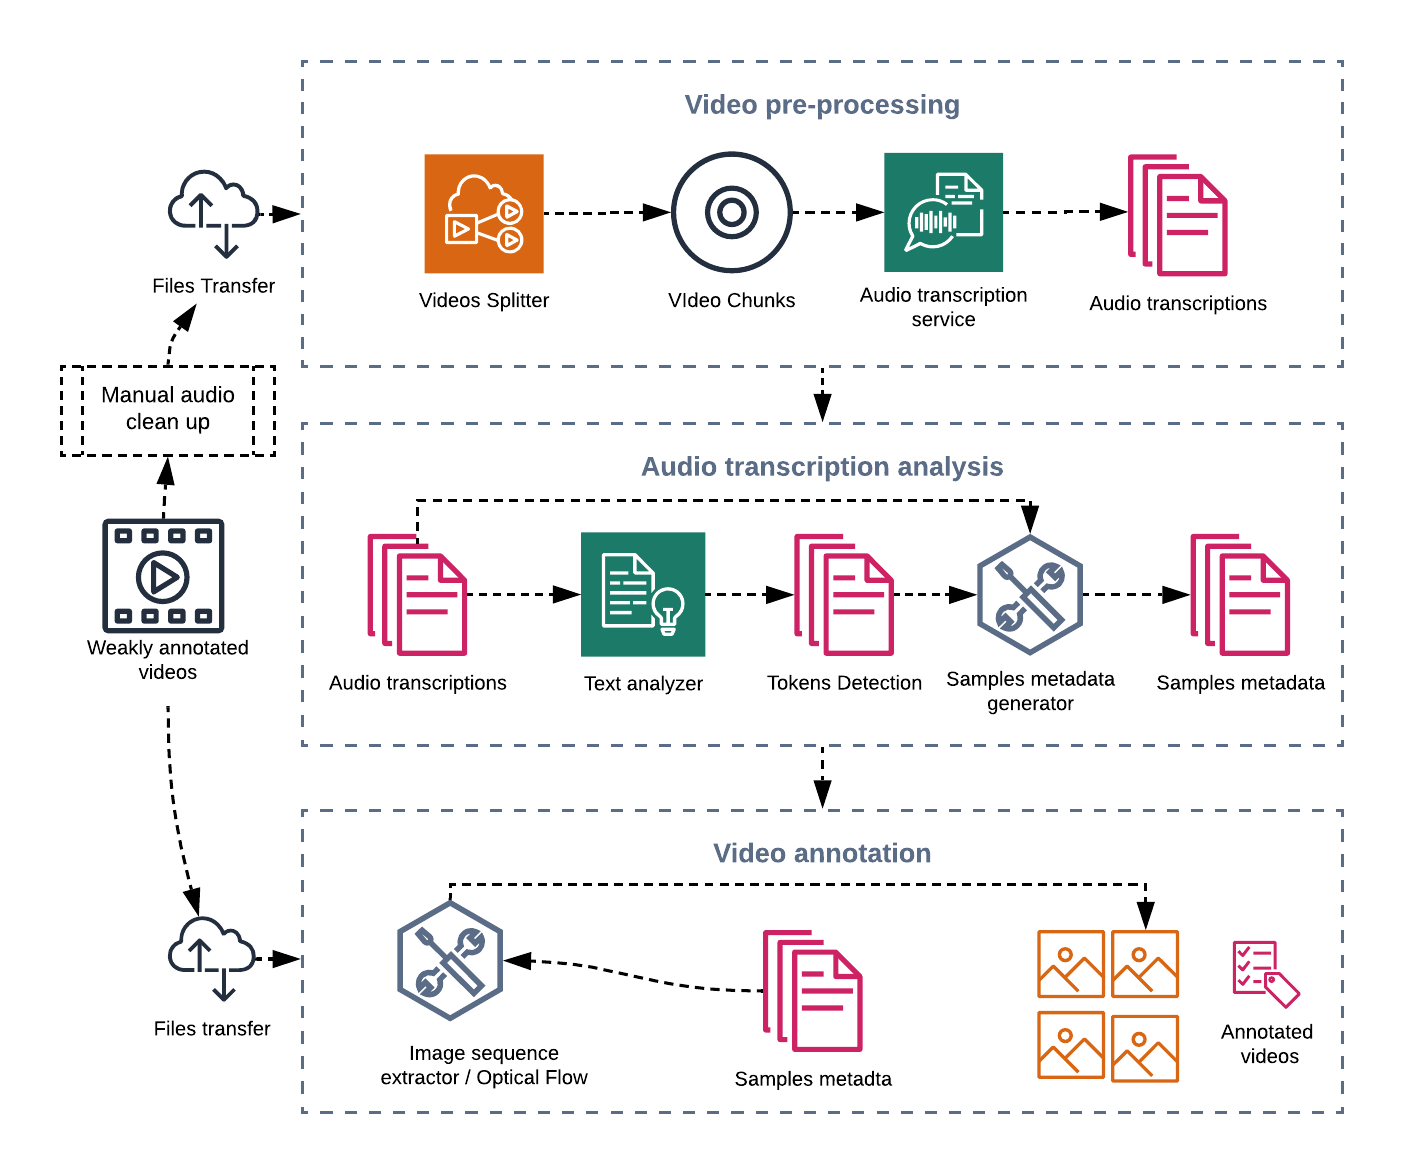
\includegraphics[width=\linewidth]{images/video-annotation-pipeline.png}
\caption{Video annotation process}
\label{fig:video-annotation-pipeline}
\end{figure}

\subsubsection{Manual Video Clean Up}\label{manual-video-cleanup}
The PSL recordings contain a considerable amount of noise introduced during the recording sessions, it makes difficult to find video intervals that clearly show a relation between signs emitted by the informant and the translation delivered by the translator, the noise factors are listed in the following list:
\begin{itemize}
	\item Multiple participants speaking during the session.
	\item Conversations between participants that are not relevant to emitted sings
	\item High frequency of silent periods 
\end{itemize}
A manual video cleanup process is required to find noise free video segments (table \ref{table:noise-free-video-segments} lists a noise free video segments), it is a long process that required watching all the videos available in the PSL dataset and manually writing in a database when an informant started emitting signs and when the translator finished delivering a translation.
\begin{table}[!htb]
\captionsetup{font=footnotesize}
\centering
\begin{tabular}{lrrc}
\toprule
\multicolumn{1}{c}{\textbf{Video}} & 
	\multicolumn{1}{c}{\textbf{Start}} &
	\multicolumn{1}{c}{\textbf{End}} &
	\multicolumn{1}{c}{\textbf{Alignment}}\\
\midrule
\multirow{5}{7.5em}{\textbf{consultant-02-session-01-part-01.mp4}} & 00:15 & 00:21 & center\\
& 00:15 & 00:21 & center\\
& 00:53 & 01:07 & center\\
& 02:43 & 02:47 & center\\
& 17:33 & 18:01 & left\\
\bottomrule
\end{tabular}
\captionsetup{font=footnotesize}
\caption{Noise free video segments extract} \label{table:noise-free-video-segments}
\end{table}
The recordings show the informant in two alignments (centered and left), the manual video clean up process also stores the informant alignment, table \ref{table:informant-alignment} shows the two available alignments, we use the alignment annotation later in the process during the video frames extraction to create the PSL annotated dataset.
\begin{table}[!htb]
\captionsetup{font=footnotesize}
\centering
\begin{tabular}{cc}
\toprule
\multicolumn{1}{c}{\textbf{Center Aligned}} & 
	\multicolumn{1}{c}{\textbf{Left Aligned}}\\
\midrule
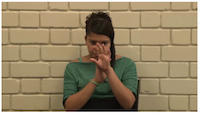
\includegraphics{images/informant-center-alignment.png}& 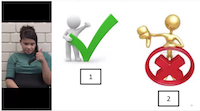
\includegraphics{images/informant-left-alignment.png}\\
\bottomrule
\end{tabular}
\caption{Informant Alignment} \label{table:informant-alignment}
\end{table}

\subsubsection{Video Pre-Processing}\label{video-pre-processing}
\subsubsection{Audio Transcription and Text Analysis}\label{audio-transcription-analysis}
\begin{table}[!htb]
\captionsetup{size=footnotesize}
\begin{tabular}{ p{16em} c}
\toprule
\multicolumn{1}{c}{\textbf{Token}} & 
	\multicolumn{1}{c}{\textbf{Frequency}}\\
\midrule
\textbf{pareja}&	4\\
\textbf{cosas}&	3\\
\textbf{cine}&	2\\
\textbf{noche}&	2\\
\textbf{terror}&	1\\
\textbf{parque}&	1\\
\textbf{casa}&	1\\
\textbf{montón}&	1\\
\textbf{apariciones}&	1\\
\textbf{fantasmas}&	1\\
\textbf{dos}&	1\\
\bottomrule
\end{tabular}
\caption{Most relevant tokens detection frequency in the PSL dataset} \label{tab:token-freq}
\end{table}

\begin{table}[!htb]
\captionsetup{font=footnotesize}
\centering
\begin{tabular}{ l p{10em} r r }
%\resizebox{\textwidth}{!}{\begin{tabular}{ llrr }
\toprule
\multicolumn{1}{c}{\textbf{Token}} & 
	\multicolumn{1}{c}{\textbf{Video}} &
	\multicolumn{1}{c}{\textbf{Start}} &
	\multicolumn{1}{c}{\textbf{End}}\\
\midrule
\textbf{cine}&	consultant-02-session-01-part-01-00.mp4&	4.19&	4.75\\
\textbf{cine}&	consultant-02-session-01-part-01-01.mp4&	1.19&	1.75\\
\textbf{terror}&	consultant-02-session-01-part-01-01.mp4&	3.82&	4.4\\
\textbf{parque}&	consultant-02-session-01-part-01-03.mp4&	8.97&	9.3\\
\textbf{casa}&	consultant-02-session-01-part-01-03.mp4&	10.12&	10.57\\
\textbf{pareja}&	consultant-02-session-01-part-01-04.mp4&	3.91&	4.36\\
\textbf{noche}&	consultant-02-session-01-part-01-04.mp4&	4.49&	4.92\\
\textbf{noche}&	consultant-02-session-01-part-01-04.mp4&	7.91&	8.2\\
\textbf{mont\'on}&	consultant-02-session-01-part-01-04.mp4&	8.5&	8.78\\
\textbf{cosas}&	consultant-02-session-01-part-01-04.mp4&	8.88&	9.38\\
\bottomrule
\end{tabular}
%\end{tabular}}
\caption{Shows metadata extacted from the PSL dataset: (1)\textit{Token} could be a noun or a number (2)\textit{Video Path} shows the video where the token was detected (3)\textit{Start Time} time when the token reproduction starts (4)\textit{End Time} time when the token reproduction ends.}
\end{table}

\subsubsection{Samples Generation}\label{samples-generation} 
\section{Conclusion}\label{conclusion}

\bibliographystyle{ieeetr}
\bibliography{References}


\end{document}
